\documentclass[12pt,a4paper]{article}
\usepackage[utf8]{inputenc}
\usepackage[german]{babel}
\usepackage[T1]{fontenc}
\usepackage{amsmath}
\usepackage{amsfonts}
\usepackage{amssymb}
\usepackage{graphicx}
\author{Florian Kluibenschedl}
\title{Direkte Analyse von Chlorophyllkataboliten}

\usepackage{chemfig,chemmacros}
\usepackage{graphicx}
\usepackage{amsmath,amssymb,amsthm,textcomp}
\usepackage{enumerate}
\usepackage{multicol}
\usepackage{tikz}
\usepackage{geometry}
\usepackage{tabu}
\usepackage{siunitx}
%\usepackage{subfig}
\usepackage{caption}
\usepackage{subcaption}
\usepackage{tabu}

\usepackage{listings}

\usepackage{rotating}
\usepackage{tabularx}

\usepackage{booktabs}
\usepackage{colortbl}
\usepackage{xcolor}
\usepackage{xfrac}
\usepackage[export]{adjustbox}[2011/08/13]

\usepackage[toc,automake]{glossaries}
% Allgemeine Abkürzungen
\newacronym{lm}{LM}{Lösungsmittel}
\newacronym{meoh}{MeOH}{Methanol}
\newacronym{eppi}{EPPI}{Eppendorf Reaktionsgefäß}
\newacronym{zB}{z.B.}{zum Beispiel}
\newacronym{bzw}{bzw.}{beziehungsweise}
\newacronym{uA}{u.a.}{unter anderem}
\newacronym{ca}{ca.}{circa}
\newacronym{nAb}{nAb.}{noch Aufklärungsbedarf}

% Chromatographie Abkürzungen
\newacronym{hplc}{HPLC}{High performance liquid chromatography}
\newacronym{rp}{RP}{Reversed-phase}
\newacronym{lcms}{LC-MS}{Liquid Chromatography-Mass Spectrometry}

% Massenspektrometrie Abkürzungen
\newacronym{EI}{EI}{Electron Ionization}
\newacronym{ESI}{ESI}{Electrosprayionisation}
\newacronym{CI}{CI}{Chemical Ionization}
\newacronym{FI}{FI}{Field Ionization}
\newacronym{mz}{m/z}{Masse pro Ladung}
\newacronym{cid}{CID}{Collision induced Dissociation}
\newacronym{pqd}{PQD}{PQD}
\newacronym{nKE}{NKE}{normalisierte Kollisionsenergie (in \%)}

% Chlorophyllkataboliten Abkürzungen
\newacronym{NCC}{NCC}{Non flourescent Chlorophyllic Catabolite}
\newacronym{YCC}{YCC}{Flourescent Chlorophyllic Catabolite}
\newacronym{DNCC}{DNCC}{Decarboxylated-Non flourescent Chlorophyllic Catabolite}
\newacronym{Chl-K}{Chl-Katabolit}{Chlorophyll Katabolit}

% chemische Formeln Abkürzungen
\newacronym{n2}{N2}{Stickstoff}
\makeglossaries

\newcommand{\mybiblatexstyle}{numeric}
\newcommand{\mybiblatexdashed}{false}  %% "true" or "false"
\newcommand{\mybiblatexbackref}{true}  %% "true" or "false"

\newcommand{\mybiblatexfile}{references-biblatex.bib}

\usepackage[backend=biber, %% using "biber" to compile references (instead of "biblatex")
style=\mybiblatexstyle, %% see biblatex documentation %% see biblatex documentation
%dashed=\mybiblatexdashed, %% do *not* replace recurring reference authors with a dash
backref=\mybiblatexbackref, %% create backlings from references to citations
natbib=true, %% offering natbib-compatible commands
hyperref=true, %% using hyperref-package references
sorting= none,
doi=true,
maxcitenames=10,
maxbibnames=100,
]{biblatex}  %% remove, if using BibTeX instead of biblatex

\addbibresource{references-biblatex.bib}

\begin{document}
\maketitle

\section{Abstract}
  Im Rahmen eines Praktikums am Organischen Institut der Universität Innsbruck wurden die Endprodukte des Abbauprozesses von Chlorophyll (Chlorophyll-Kataboliten) frisch gepflückter Brokkoliblätter einer direkten Analyse mit MS-Leafspray unterzogen.\\

MS-Leafspray stellt dabei eine neue, moderne Methode der Massenspektrometrie dar, die es ermöglicht, Probenmaterial in natürlicher Umgebung zu analysieren. Nach einer Erstidentifikation über MS-Leafspray wurde das Ergebnis mit LC-MS verifiziert. Die mit beiden Methoden gefundenen Chlorophyll-Kataboliten lauten wie folgt: \textit{Bo}-NCC-1, \textit{Bo}-NCC-3, \textit{Bo}-DNCC, \textit{Bo}-DNCC-2, \textit{Bo}-DYCC und \textit{Bo}-YCC. Im Vergleich zur Brokkolifrucht konnten vier weitere Chlorophyll-Kataboliten gefunden werden, was neue Fragen in Bezug auf das Verständnis des Abbauprozesses aufwirft. 

Ebenso konnten die Reaktionsprodukte einer Reaktion am Blatt mit Essigsäureanhydrid mithilfe von MS-Leafspray nachgewiesen werden. Auf Basis diverser Fragmentierungen wird vorgeschlagen, dass die Reaktion nur an einer der beiden freien Carbonsäuren der Chlorophyll-Kataboliten erfolgt. 

Im Rahmen der massenspektrometrischen Analysen wurden Fragmentierungsdiagramme erstellt, von denen angesichts der Ergebnisse vermutet wird, dass sie charakteristisch für bestimmte Chlorophyll-Kataboliten sind. Eine Interpretationsmöglichkeit der Diagramme wurde vorgeschlagen.

\section{Einleitung}

Jedes Jahr werden weltweit schätzungsweise $10^{9}$ Tonnen an Chlorophyll abgebaut. Der Abbauprozess des Chlorophylls ist damit aufgrund der markanten Farbveränderungen einer der visuell am meisten wahrgenommenen biochemischen Vorgänge und kann sogar aus dem All beobachtet werden. \cite{ChlorophyllBreakdown} Die schönen, bunten Farben des Herbstlaubes werden dabei jedoch nicht primär durch die Abbauprodukte des Chlorophylls (Chlorophyll-Kataboliten) hervorgerufen  \cite{DegradationChlorophyll}, da die Endprodukte des Chlorophyllabbaus zumeist farbblos sind. \cite{ChlorophyllBreakdown} Die Abbauprodukte fallen in die Klasse der Phyllobiline (heterocyclische Tetrapyrrole) und sind Anzeichen für Reifung, Seneszenz und Zelltod. Der Abbauprozess wird unter anderem im Rahmen eines Entgiftungsprozesses begangen. \cite{ChlorophyllKatabolitenalsZeichenReifung}

\begin{figure}[!hbtp]
  \centering
  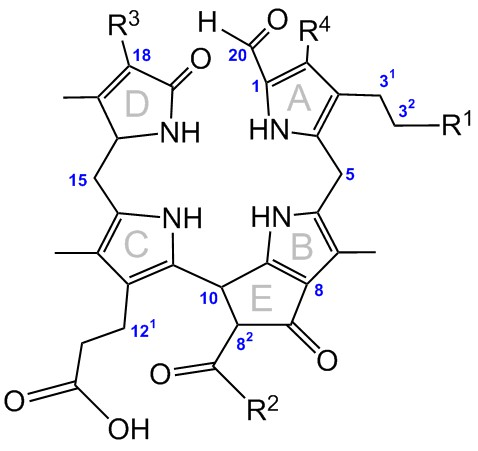
\includegraphics[scale=0.5]{figures/Kapitel2/VWA_Chl-Nummerierung.png}
  \caption[Nummerierung von Phyllobilinen, Quelle: Autor]{Beispiel eines Phyllobilins inklusive Positionsangaben und Bezeichnungen der Ringe, an den mit Rest (R) gekennzeichneten Stellen werden strukturelle Unterschiede beobachtet}
  \label{fig:NummerierungPhyllobiline}
\end{figure}

Die unterschiedlichen Arten an Chl-Kataboliten ergeben sich durch Anlagerungen der entsprechenden funktionellen Gruppen (z. B. Zuckerring, Hydroxygruppe) an den pFCC, der ein Zwischenprodukt im komplexen Abbauprozess darstellt. \cite{ChlorophyllCatabolites} \\

Das Ziel dieser Arbeit bestand darin, die Chl-Kataboliten des Brokkoliblattes mithilfe von MS-Leafspray zu analysieren. MS-Leafspray ist dabei eine massenspektrometrische Methode, Proben mithilfe von \textit{Ambient Ionization} \cite{AmbientIonisation} in ihrer \textit{natürlichen} Umgebung zu analysieren. Leaf Spray ist eine Form von Paper Spray \cite{PaperSpray}, bei der die zu analysierende Pflanze selbst als poröses Material dient. Die mit MS-Leafspray erhaltenen Ergebnisse wurden mit LC-MS und einem hochauflösendem Massenspektrometer überprüft.

\pagebreak

\section{Experimenteller Teil}

\subsection{Versuchsaufbau MS-Leafspray} \label{sec:Versuchsaufbau}

%Abbildung \ref{fig:LeafsprayVersuchsaufbau} beschreibt schematisch den Versuchsaufbau. 

\begin{figure}[!hbtp]
  \centering
  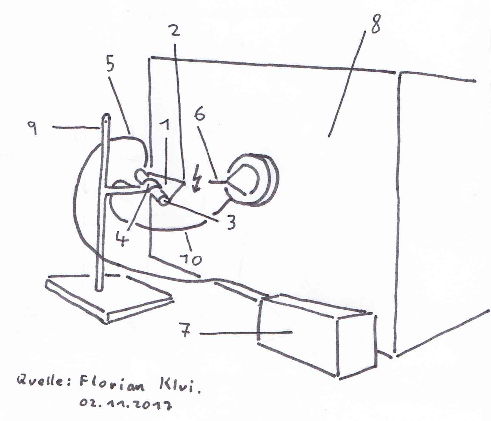
\includegraphics[scale=0.5]{figures/Kapitel4/VWA_MSLeafspray_Versuchsaufbau.png}
  \caption[MS Leafspray Versuchsaufbau, Quelle: Autor]{Leafspray Versuchsaufbau: 1) Filterpapierdreick, 2) Spitze des Dreiecks, 3) Blattmaterial, von Filterpapier umschlossen, 4) Kupferklemme, 5) Kapillare für \gls{lm}, 6) Einlass des Massenspektrometers (mit der markanten Spitze zwecks Verdeutlichung etwas übertrieben dargestellt), 7) \textit{Syringe Pump} - kontrolliert den \gls{lm}-Fluss durch 5), 8) Ionenfallen Massenspektrometer, 9) Stativ, 10) Kabel, mit 4) verbunden - zwischen 4) und 6) liegt eine Spannung   an (3-6 kV - durch Blitz zwischen 2) und 6) symbolisiert)}
  \label{fig:LeafsprayVersuchsaufbau}
\end{figure}

Die im Folgenden beschriebene Versuchsdurchführung erwies sich als besonders effizient:

Das zu analysierende Blatt wurde zugeschnitten und in Filterpapier eingerollt. Das Filterpapierdreieck wurde in einer Kupferklemme eingespannt. Die Kupferklemme wurde mit einem Kabel (10), das an einem Ionenfallen Massenspektrometer (8) angeschlossen war, verbunden. Zwischen der Kupferklemme (4) und dem Massenspektrometer wurde eine Spannung von 3-6 kV angelegt. Da das Filterpapier mit \gls{lm} benetzt ist und eine Verbindung der Flüssigkeit zur Kupferklemme besteht, kommt es zu einer durch die Spannung ausgelösten Bewegung der im \gls{lm} gelösten Ionen, die in geladenen Tröpfchen in das Massenspektrometer hineinfliegen. Der Abstand zwischen Filterpapier (2) und Einlass des Massenspektrometers (6) betrug ungefähr 0.5 cm.

\begin{figure}[htbp]
  \begin{subfigure}[b]{0.5\textwidth}
    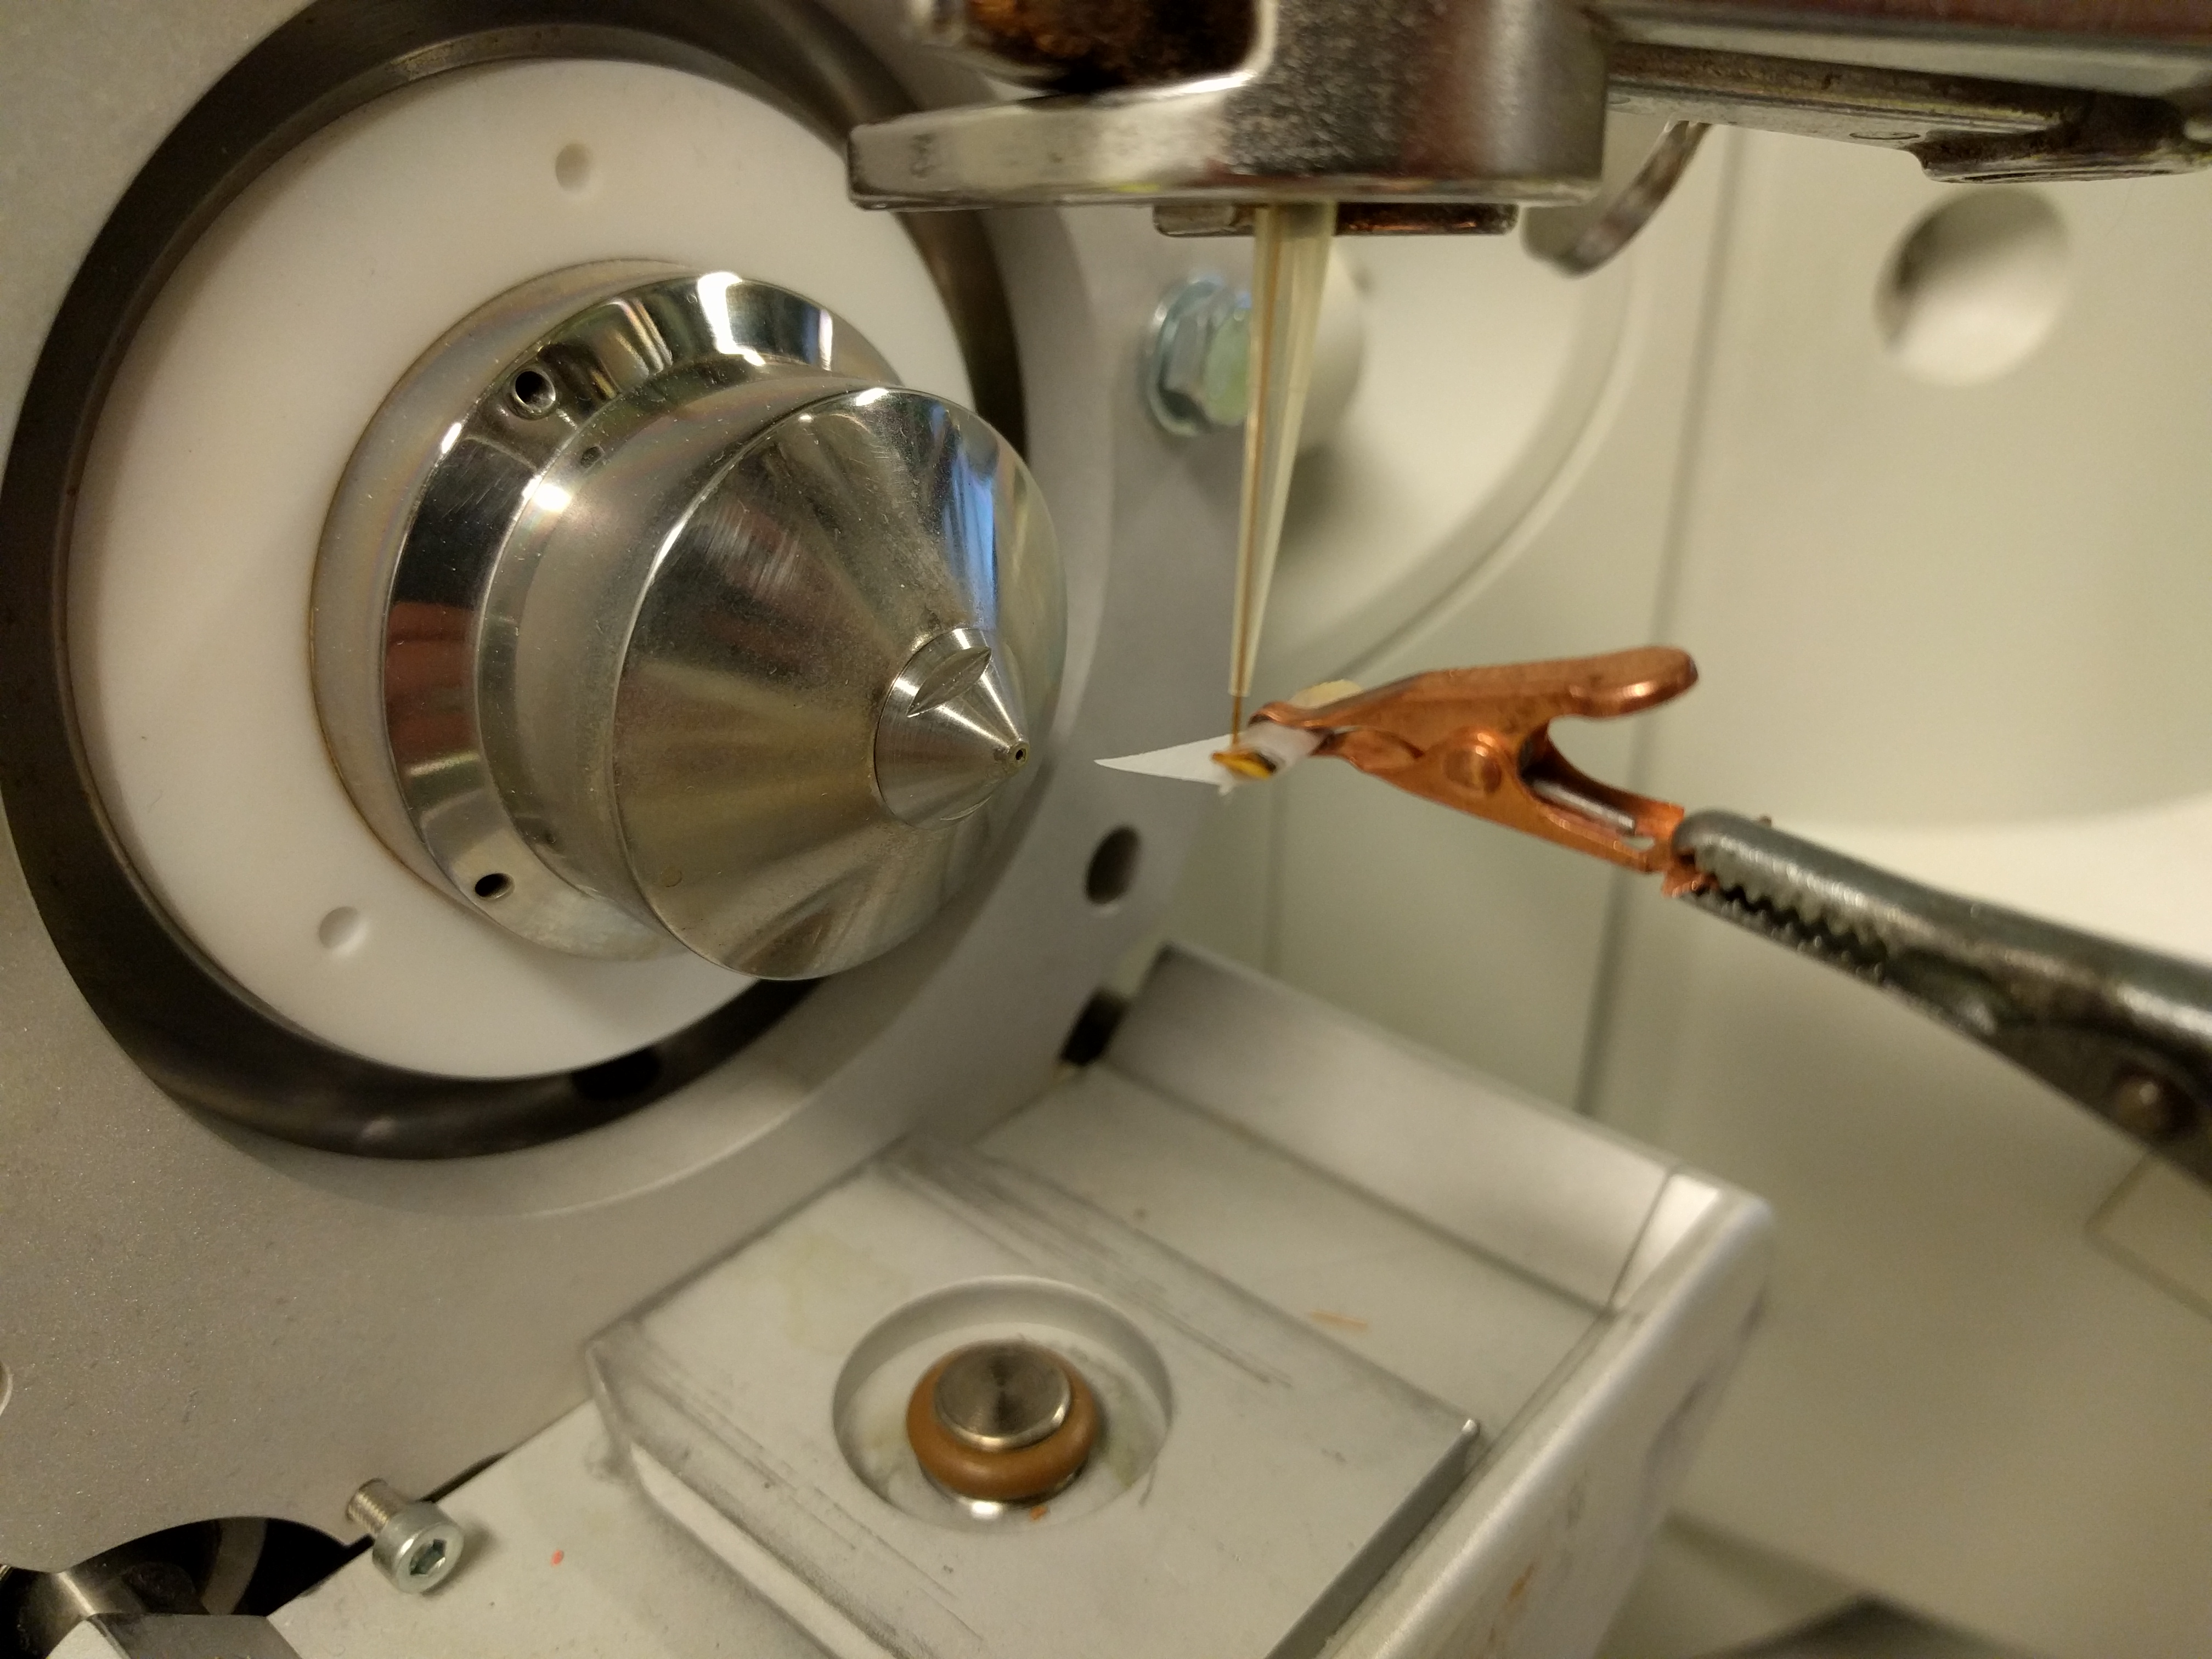
\includegraphics[width=\textwidth]{figures/Kapitel4/VWA_MSLeafspray_Detail1.jpg}
    \caption{}
    \label{fig:MSLeafsprayDetail1}
  \end{subfigure}
  \hfill
  \begin{subfigure}[b]{0.5\textwidth}
    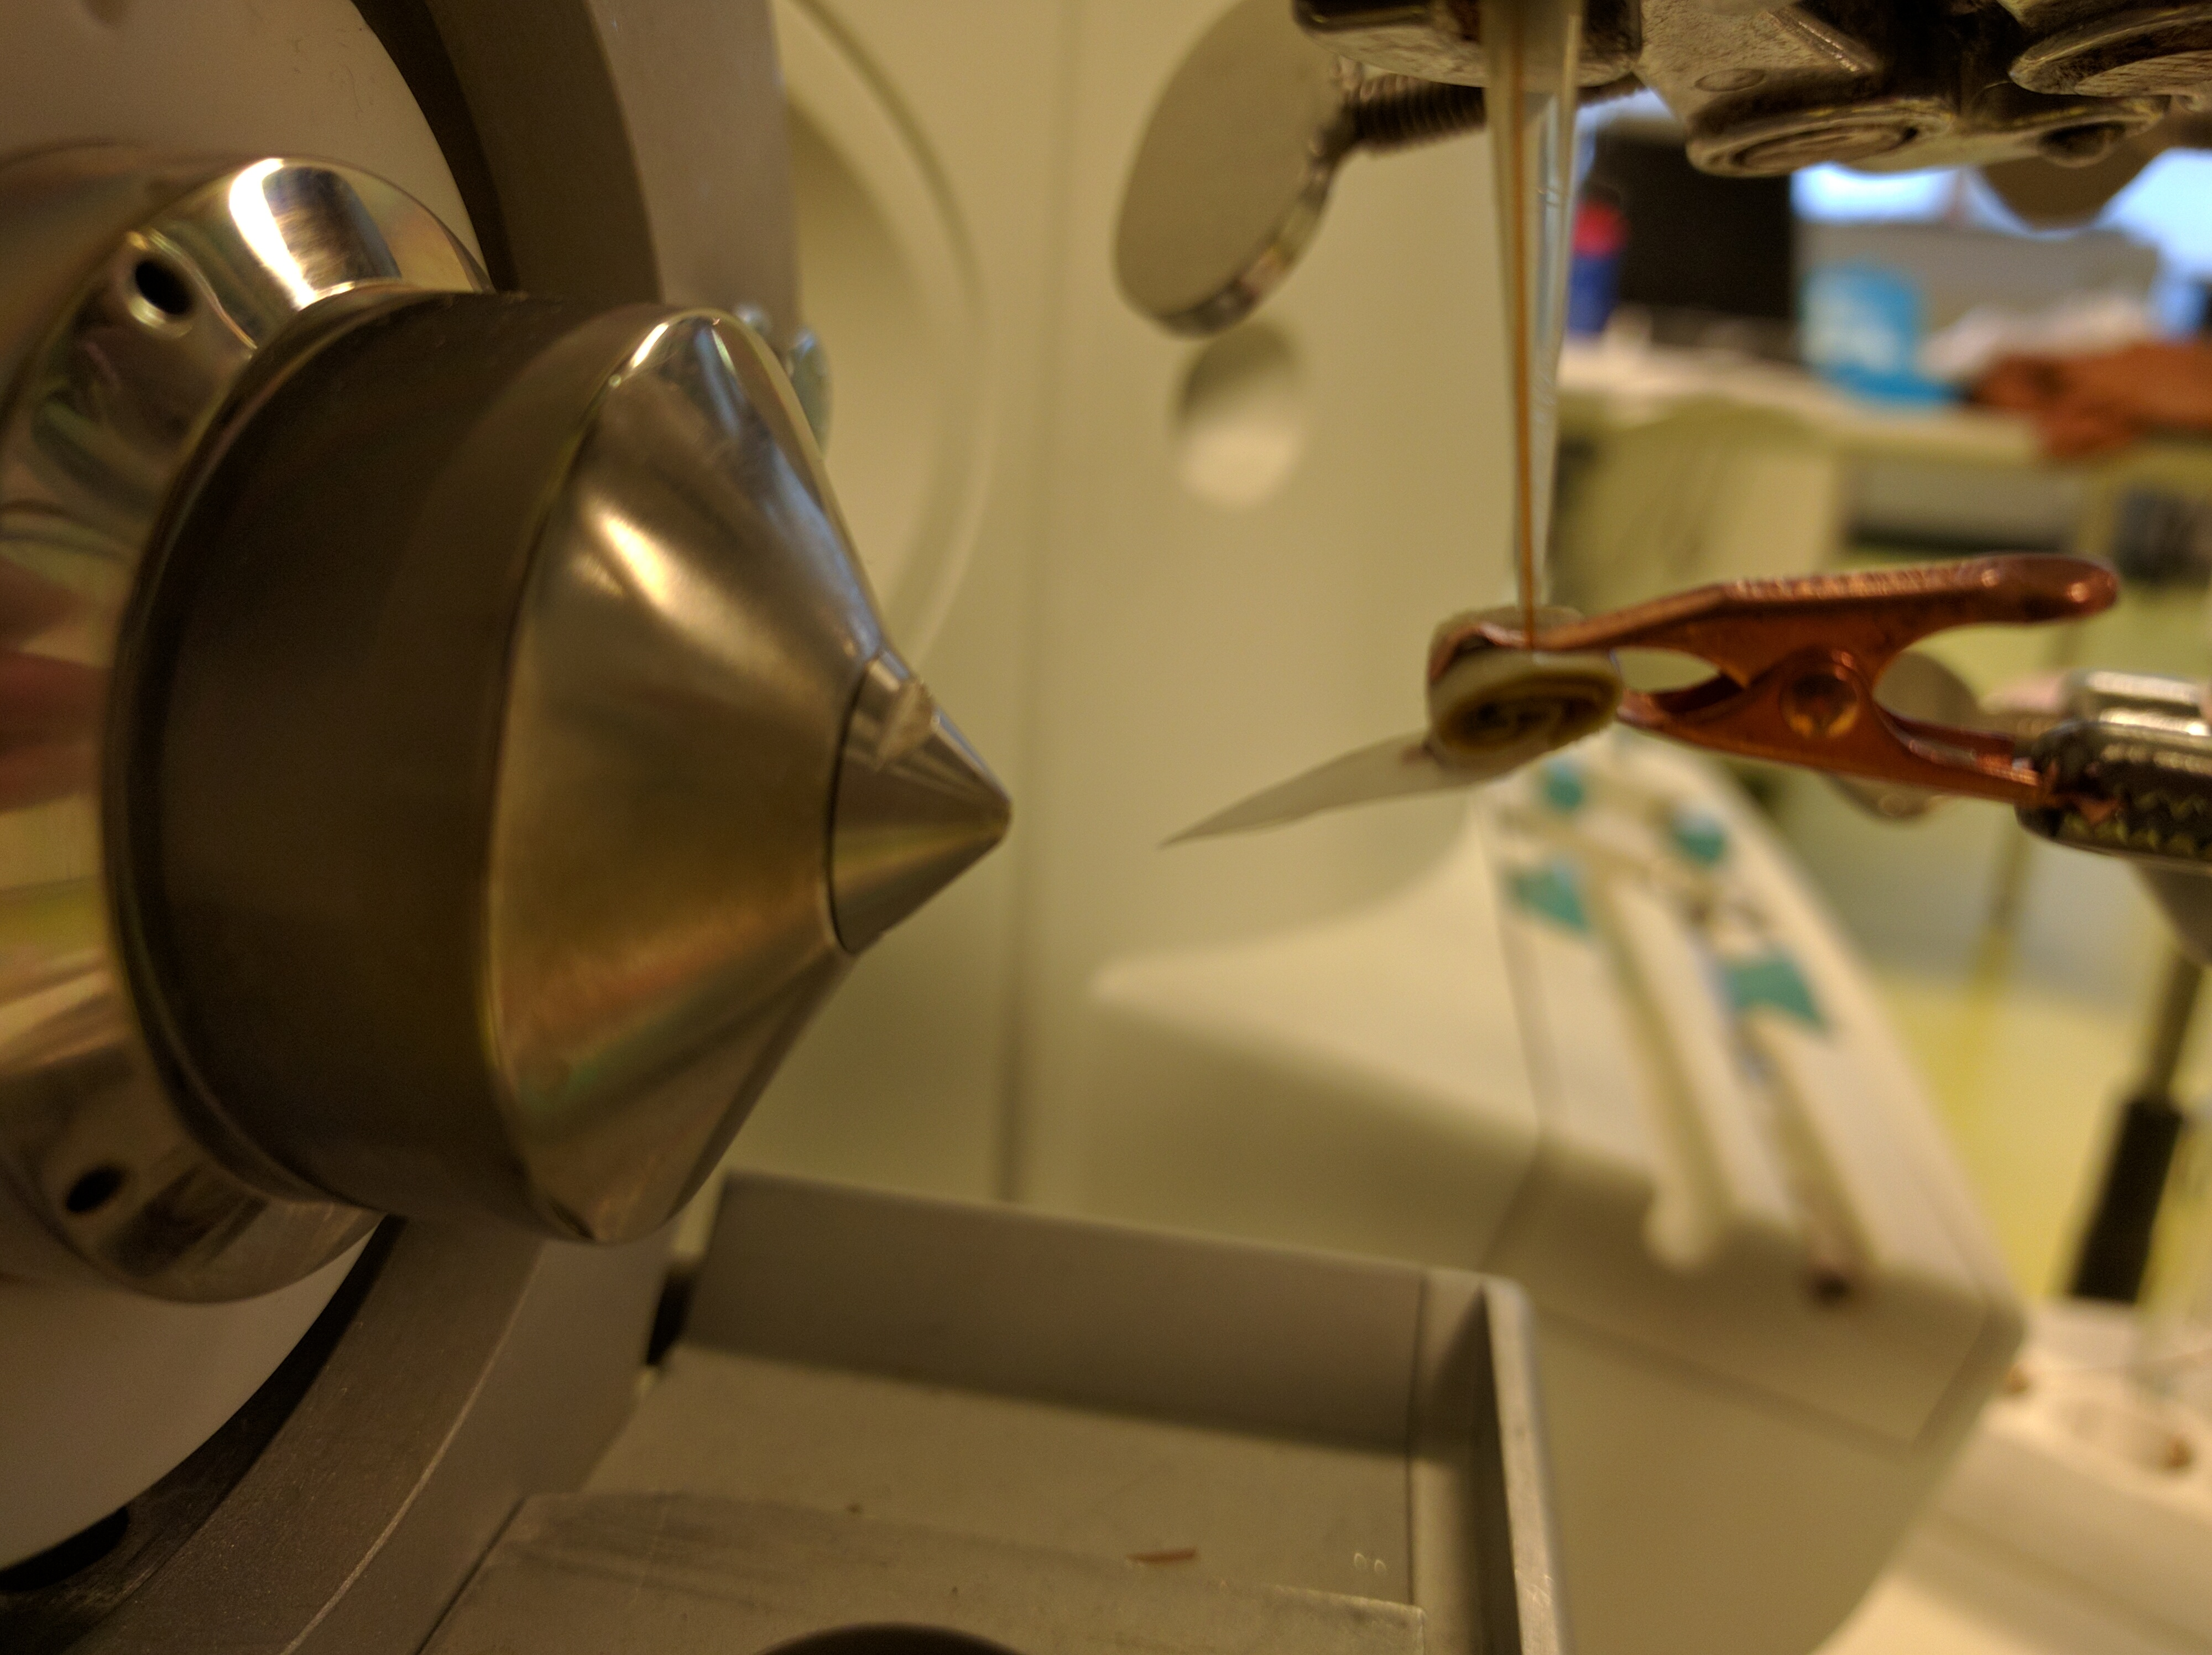
\includegraphics[width=\textwidth]{figures/Kapitel4/VWA_MSLeafspray_Detail2.jpg}
    \caption{}
    \label{fig:MSLeafsprayDetail2}
  \end{subfigure}
  \caption[MS Leafspray Versuchsaufbau Detailfotos, Quelle: Autor]{(a) Einlass des Massenspektrometers mit Kapillare (5), Kupferklemme (4) und Filterpapier mit Blattmaterial (1) und (3), (b) Detailansicht}
  \label{fig:MSLeafsprayDetail}
\end{figure}

In Abbildung \ref{fig:MSLeafsprayDetail} wird gezeigt, wie diese Anordnung umgesetzt wurde. Zu sehen sind die Kupferklemme mit dem eingespannten Filterpapier und dem darin enthaltenen Blatt, die \gls{lm}-Kapillare, die Einlassöffnung des Massenspektrometers und der Abstand von Filterpapierdreieckspitze zum Massenspektrometer. Es gilt zu beachten, dass das Filterpapier in einem gewissen Winkel eingespannt wurde (Abbildung \ref{fig:MSLeafsprayDetail2}), um zu verhindern, dass das \gls{lm} nicht abfließt, was bei einer waagrechten Anordnung in Form einer \textit{Sackbildung} des LM auftreten kann.

\section{Resultate}

In Tabelle \ref{tab:LCMSKatabolitenRPListe} sind alle Chl-Kataboliten aufgelistet, die mithilfe von MS-Leafspray und LC-MS identifiziert werden konnten. Da im Zuge der Versuche eine Reaktion der Chl-Kataboliten mit Essigsäureanhydrid durchgeführt wurde, werden auch die Reaktionsprodukte genannt. Das Edukt wird in der entsprechenden Spalte aufgelistet.

\begin{sidewaystable*}[!htbp]\centering
  %\ra{1.3}
  
  \begin{tabular}{ccccccccc}\toprule
 Chl-Katabolit & Summenformel & [M+H]\textsuperscript{+} & MS-Leafspray & Typ & HPLC & Edukt \\
\midrule
\rowcolor{black!20} \textit{Bo}-DYCC & \ch{C33H37O8N4} & 617.2599 & x & DYCC & 30.94? & -\\
 \textit{Bo}-DNCC & \ch{C33H39O8N4} & 619.2798 & 657 & DNCC & 26.72 & -\\ 
\rowcolor{black!20} • & \ch{C34H37O8N4} & 629.2641 & x & • & - & -\\ 
 - & \ch{C34H39O8N4} & 631.2795 & x & DYCC & 29.91, 30.94 & \textit{Bo}-DYCC\\ 
\rowcolor{black!20} - & \ch{C34H41O8N4} & 633.2955 & x & DNCC & 28.8 & \textit{Bo}-DNCC\\ 
 • & \ch{C36H33O7N4} & 633.2339 & x & • & - & -\\ 
\rowcolor{black!20} \textit{Bo}-YCC & \ch{C34H37O9N4} & 645.2593 & x & YCC & - & -\\ 
 - & \ch{C35H41O8N4} & 645.2953 & x & DYCC & - & \textit{Bo}-DYCC\\ 
\rowcolor{black!20} \textit{Bo}-NCC-3 & \ch{C34H39O9N4} & 647.2748 & 685 & NCC & 33.04 & -\\ 
 • & \ch{C34H35O10N4} & 659.2348 & x & • & - & -\\
\rowcolor{black!20} - & \ch{C35H39O9N4} & 659.2741 & x & YCC & 37.09 & \textit{Bo}-YCC\\
 - & \ch{C35H41O9N4} & 661.2902 & x & NCC & - & \textit{Bo}-NCC-3\\
\rowcolor{black!20} - & \ch{C36H43O9N4} & 675.306 & x & NCC & - & \textit{Bo}-NCC-3\\
 \textit{Bo}-DNCC-2 & \ch{C39H47O13N4} & 779.3181 & x & DNCC & - & -\\ 
\rowcolor{black!20} \textit{Bo}-NCC-1 & \ch{C40H49O13N4} & 793.3336 & 831 & NCC & 29.91 & -\\ 
 - & \ch{C40H51O13N4} & 795.3491 & x & - & - & -\\ 
\rowcolor{black!20} - & \ch{C41H51O13N4} & 807.3491 & x & NCC & 40.03 & \textit{Bo}-NCC-1\\ 
 - & \ch{C41H53O13N4} & 809.3649 & x & - & - & 795\\ 
\rowcolor{black!20} - & \ch{C42H53O13N4} & 821.3652 & x & NCC & 47.28 & \textit{Bo}-NCC-1\\ 
 - & \ch{C35H41N4O9}* & x & 699 & DNCC* & - & \textit{Bo}-DNCC \\ 
\rowcolor{black!20} - & \ch{C36H40N4O10}* & x & 727 & & NCC* & \textit{Bo}-NCC-3\\ 
 - & \ch{C42H50N4O14}* & x & 873 & NCC* & - & \textit{Bo}-NCC-1 \\ 
\bottomrule
  \end{tabular}
  
  \caption[Übersicht über die Chl-Kataboliten des Brokkoliblattes unter Berücksichtigun der Erkenntnisse aller Methoden, Quelle: Autor]{Übersicht über die gefundenen Chl-Kataboliten des Brokkoliblattes und ihren Reaktionsprodukten}
  \label{tab:LCMSKatabolitenRPListe}
\end{sidewaystable*}

\subsection{Chl-Kataboliten mit MS-Leafspray identifiziert}

Mithilfe von MS-Leafspray konnten ein \textit{Bo}-NCC-1, \textit{Bo}-NCC-3 sowie ein \textit{Bo}-DNCC identifiziert werden. Die anderen in Tabelle \ref{tab:LCMSKatabolitenRPListe} aufgelisteten Verbindungen wurden mit LC-MS analysiert. Zu den besagten Chl-Kataboliten wurden sogenannte Fragmentierungsdiagramme erstellt. Bei diesen wird die gemessene Intensität der Fragmentierungen gegen die aufgewendete, normalisierte Kollisionsenergie (nKE), aufgetragen.\footnote{die erhaltenen Kurven wurden mit einem Savitzky-Golay Filter geglättet \cite{scipy}, weswegen manche Graphen der Fragmentierungen nicht im Ursprung starten} Unter anderem zeigen sie, dass ab einer bestimmten nKE (ca. 50 nKE) die Anregung so stark ist, dass das Molekül fast komplett zerfällt, weswegen fast keine Fragmente beobachtet werden können. Es bleibt noch zu klären, ob die Fragmentierungsdiagramme charakteristisch für einen Chl-Kataboliten sind. 

\begin{figure}[!htbp]
  \begin{subfigure}[b]{0.5\textwidth}
    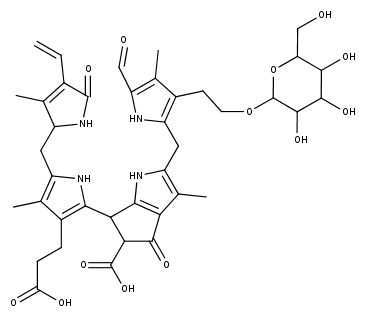
\includegraphics[width=\textwidth]{figures/Kapitel4/Kataboliten/fragmentation_structures/VWA_Katabolit_831.png}
    \caption{}
    \label{fig:831MKLeafspraystructure}
  \end{subfigure}
  \hfill
  \begin{subfigure}[b]{0.7\textwidth}
    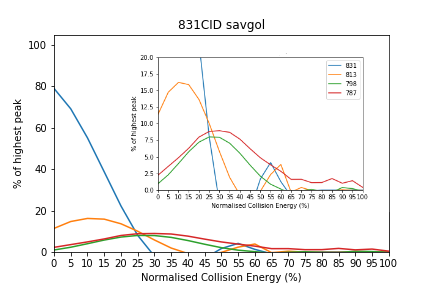
\includegraphics[width=\textwidth]{figures/Kapitel4/Kataboliten/diags/831CID-savgol.png}
    \caption{}
    \label{fig:831MKLeafspraydiags}
  \end{subfigure}
  \caption[Strukturvorschlag des \textit{Bo}-NCC-1 und Fragmentierungsdiagramm, Quelle: Autor]{(a) Strukturvorschlag des \textit{Bo}-NCC-1 mit Summenformel \ch{C40H48N4O13}, (b) Fragmentierungsdiagramm von \textit{Bo}-NCC-1 (blau = 831 [M+K]\textsuperscript{+}, orange = 813 [M - \ch{H2O} + K]\textsuperscript{+}, grün = 798 [M - (\ch{MeOH} - \gls{nAb}) + K]\textsuperscript{+}, rot = 787 [M - \ch{CO2} + K]\textsuperscript{+})}
\end{figure}

Die Reaktionsprodukte der Reaktion mit Essigsäureanhydrid konnten ebenfalls mit MS-Leafspray identifiziert werden, wobei Acetonitril als Lösungsmittel verwendet wurde. Mit LC-MS konnten nicht die Anhydride, sondern lediglich die Methylester beobachtet werden, da Methanol als LM verwendet wurde. 

Ein Strukturvorschlag des Reaktionsproduktes von \textit{Bo}-NCC-1 wird in Abbildung \ref{fig:873MKstructure} gemacht. Das dazugehörige Massenspektrum des [M+K]\textsuperscript{+} Ions wird in Abbildung \ref{fig:873MKLeafspray} dargestellt. Zu sehen sind die Abspaltungen von \ch{H2O} bei m/z = 855 [M - \ch{H2O} + K]\textsuperscript{+}, von Essigsäure bei m/z = 813 [M - \ch{CH3COOH} + K]\textsuperscript{+} und von \ch{CH3COOH}, Ring A, Ring D, zweimal MeOH und CO bei m/z = 309 [M - (\ch{CH3COOH}, Ring A, Ring D, 2 x MeOH, CO) + K]\textsuperscript{+}.\footnote{Die zuletzt genannte Abspaltungsfolge muss noch im Rahmen weiterer Untersuchungen bestätigt werden. Im Moment handelt es sich um einen möglichen Vorschlag.}

\begin{figure}[htbp]
  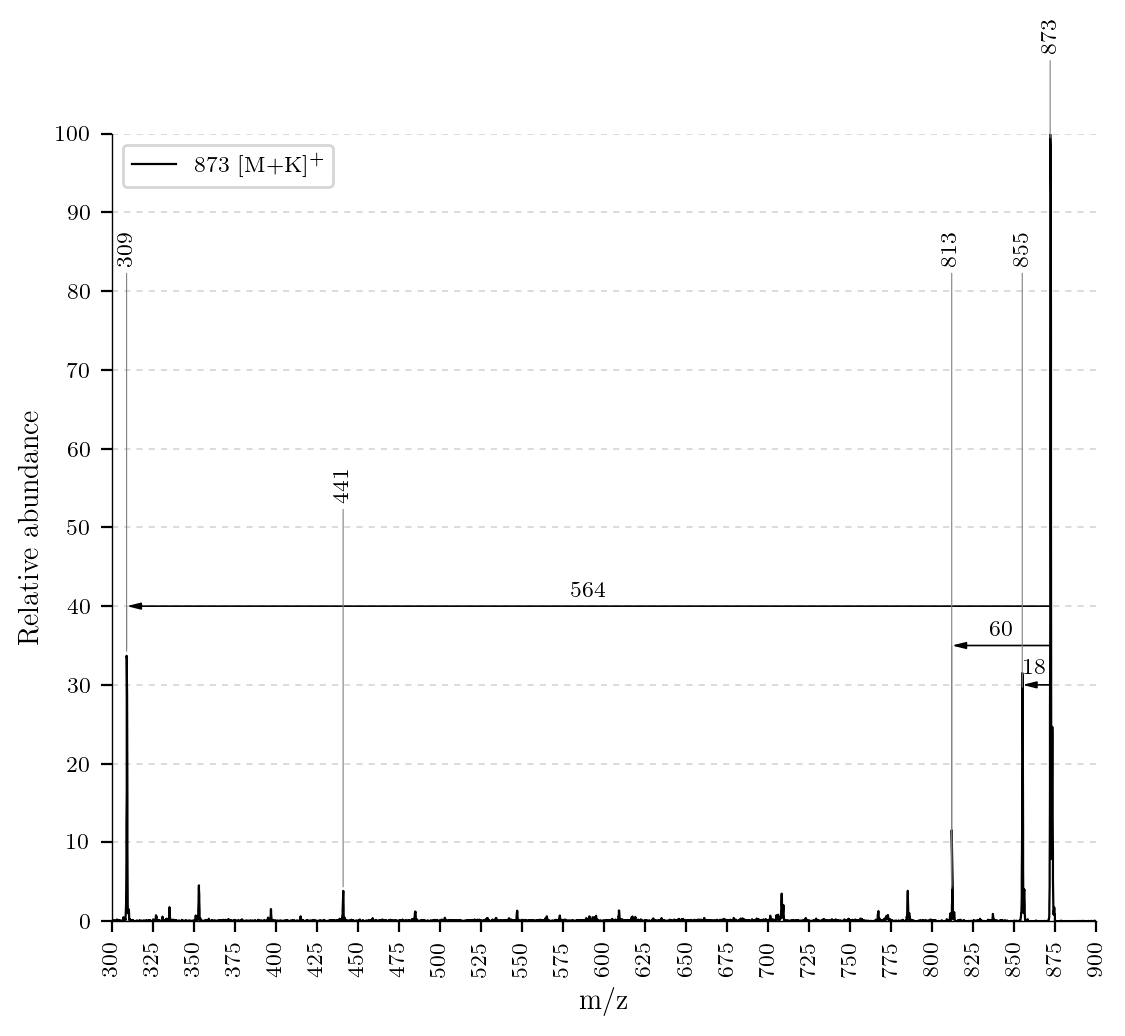
\includegraphics[width=\textwidth, height=0.7\textwidth]{figures/Kapitel4/Kataboliten/VWA_MS_LeafSpray_873.png} 
  \caption[ESI-MS des Reaktionsproduktes von \textit{Bo}-NCC-1, Quelle: Autor]{ESI-MS des Reaktionsproduktes von \textit{Bo}-NCC-1 bei m/z = 873 [M+K]\textsuperscript{+}}
  \label{fig:873MKLeafspray}
\end{figure}

\begin{figure}[htbp]
  \centering
  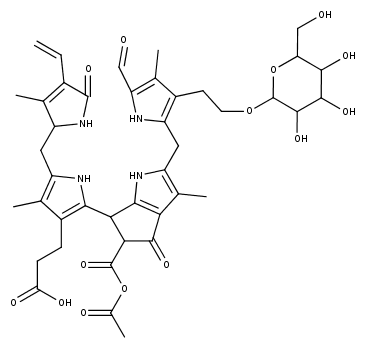
\includegraphics[scale=0.6]{figures/Kapitel4/Kataboliten/fragmentation_structures/VWA_Katabolit_873.png}
  \caption[Strukturvorschlag des Reaktionsproduktes von \textit{Bo}-NCC-1, Quelle: Autor]{Strukturvorschlag des Reaktionsproduktes von \textit{Bo}-NCC-1 mit Summenformel \ch{C42H50N4O14}}
  \label{fig:873MKstructure}
\end{figure}

\pagebreak
\subsection{Diskussion}

Im Rahmen der experimentellen Untersuchungen konnte somit der Großteil der Forschungsfragen behandelt werden. MS-Leafspray erwies sich dabei als eine zuverlässige, moderne Analysenmethode, die eine schnelle Identifikation der Chl-Kataboliten erlaubt. Besonders die weitere Erforschung der Fragmentierungsdiagramme zeigt sich als geeignet, die Strukturaufklärung mit dem Massenspektrometer noch weiter zu verbessern. So ist es unter anderem auch denkbar, dass man Rückschlüsse auf die exakte Stereochemie anstellen kann.

\printbibliography
\listoffigures

\end{document}